
\section{Conceitualização}

\subsection{Síntese de Programas}
\begin{frame}{O que é Síntese de Programas (SP)?}
    \begin{itemize}
      \item Processo de descoberta automático de programas \cite{gulwani2017}.
      \item \textit{Sem interferência humana!}
    \end{itemize}
\end{frame}

\begin{frame}{Caracterização de SP}
    \begin{itemize}
        \item Podemos caracterizar um sistema de Síntese de Programas sob 3 eixos \cite{gulwani2010}:
        \begin{itemize}
            \item Forma da especificação do problema (ou como o usuário representa sua intenção).
            \item Espaço de busca (todos os programas possíveis em uma dada representação).
            \item Heurística de busca (como navegar o espaço dos programas).
        \end{itemize}
    \end{itemize}
\end{frame}

\subsection{Programação Genética}
\begin{frame}{O que é Programação Genética (GP)?}
        \begin{itemize}
          \item Variação de algoritmos genéticos \cite{kozabook1}.
            \item Heurística baseada na ideia de evolução do mais apto.
            \item Indivíduos são programas, conjuntos de instruções seus genes.
            \item Indivíduos que produzem resultados melhores se reproduzem.
            \item Utilizado como técnica de busca em SP.
        \end{itemize}
\end{frame}
\begin{frame}{O que é Programação Genética (GP)?}
        \begin{figure}
            \centering
            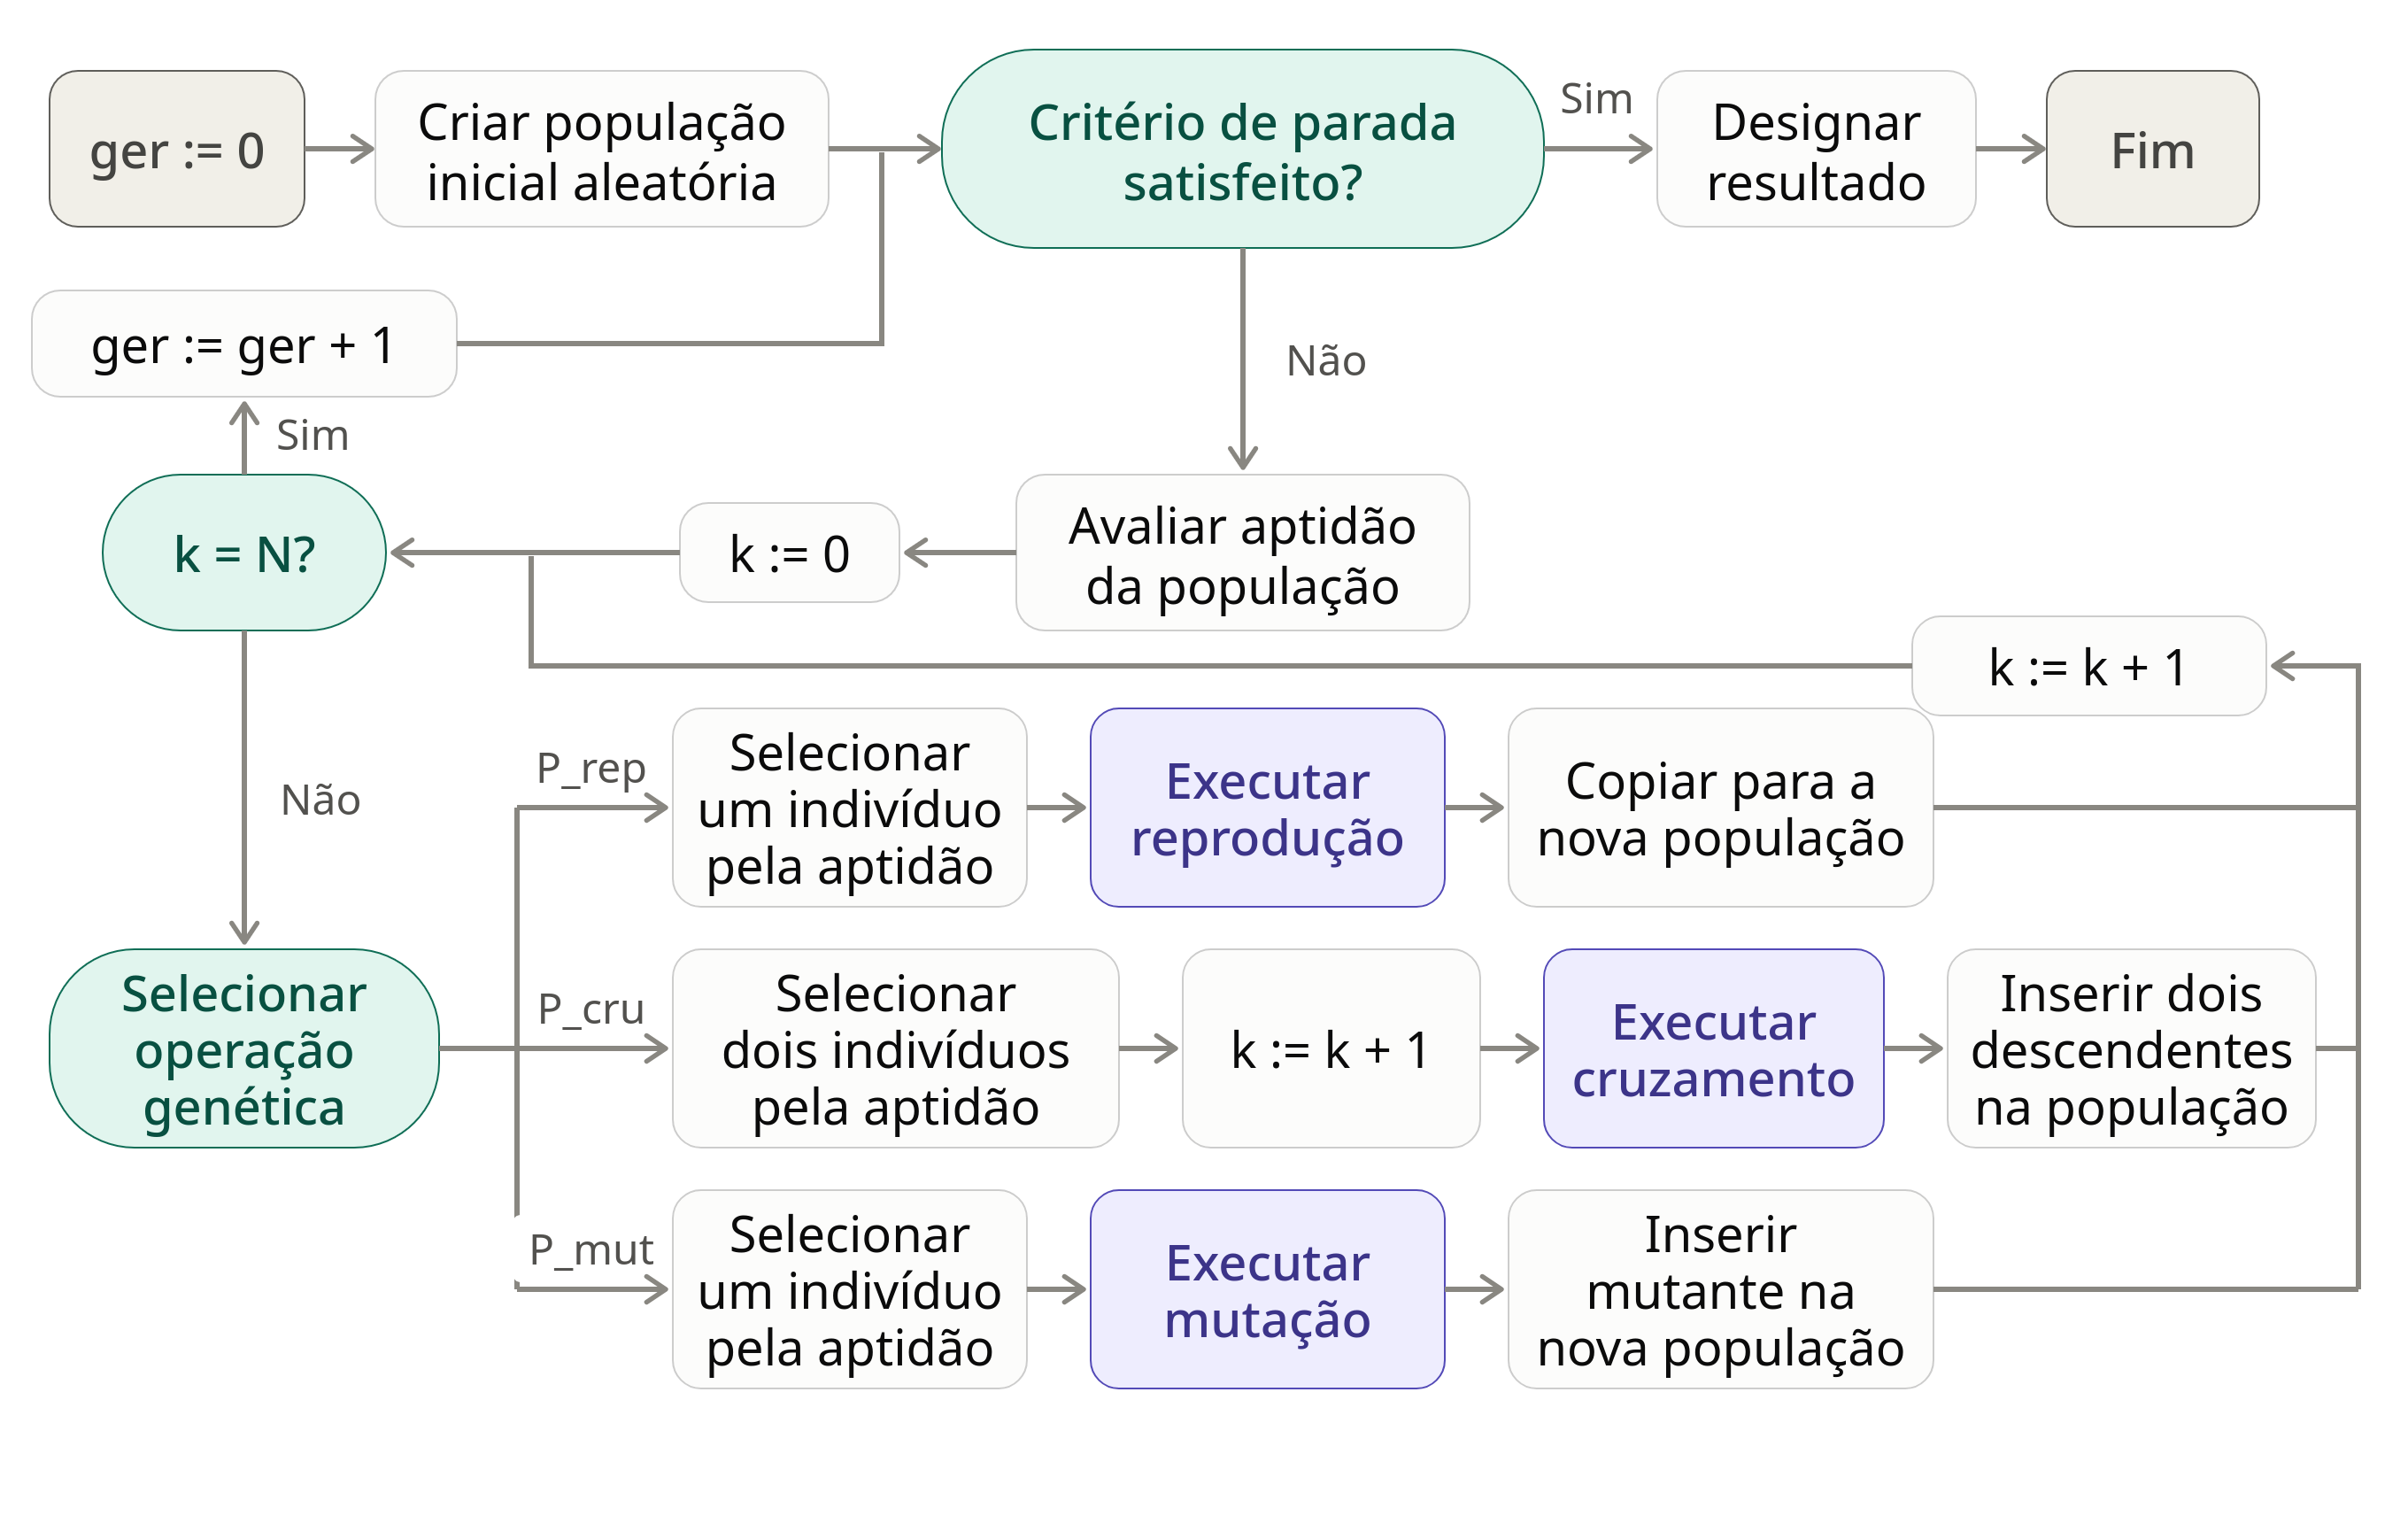
\includegraphics[width=0.7\linewidth]{imgs/flow.png}
            \caption{Fluxograma de GP. Adaptado de \cite{kozabook1}}
            \label{fig:flow}
        \end{figure}
\end{frame}
\begin{frame}{O que é Programação Genética (GP)?}
  \begin{columns}
    \begin{column}{0.5\textwidth}
      \begin{figure}
          \centering
          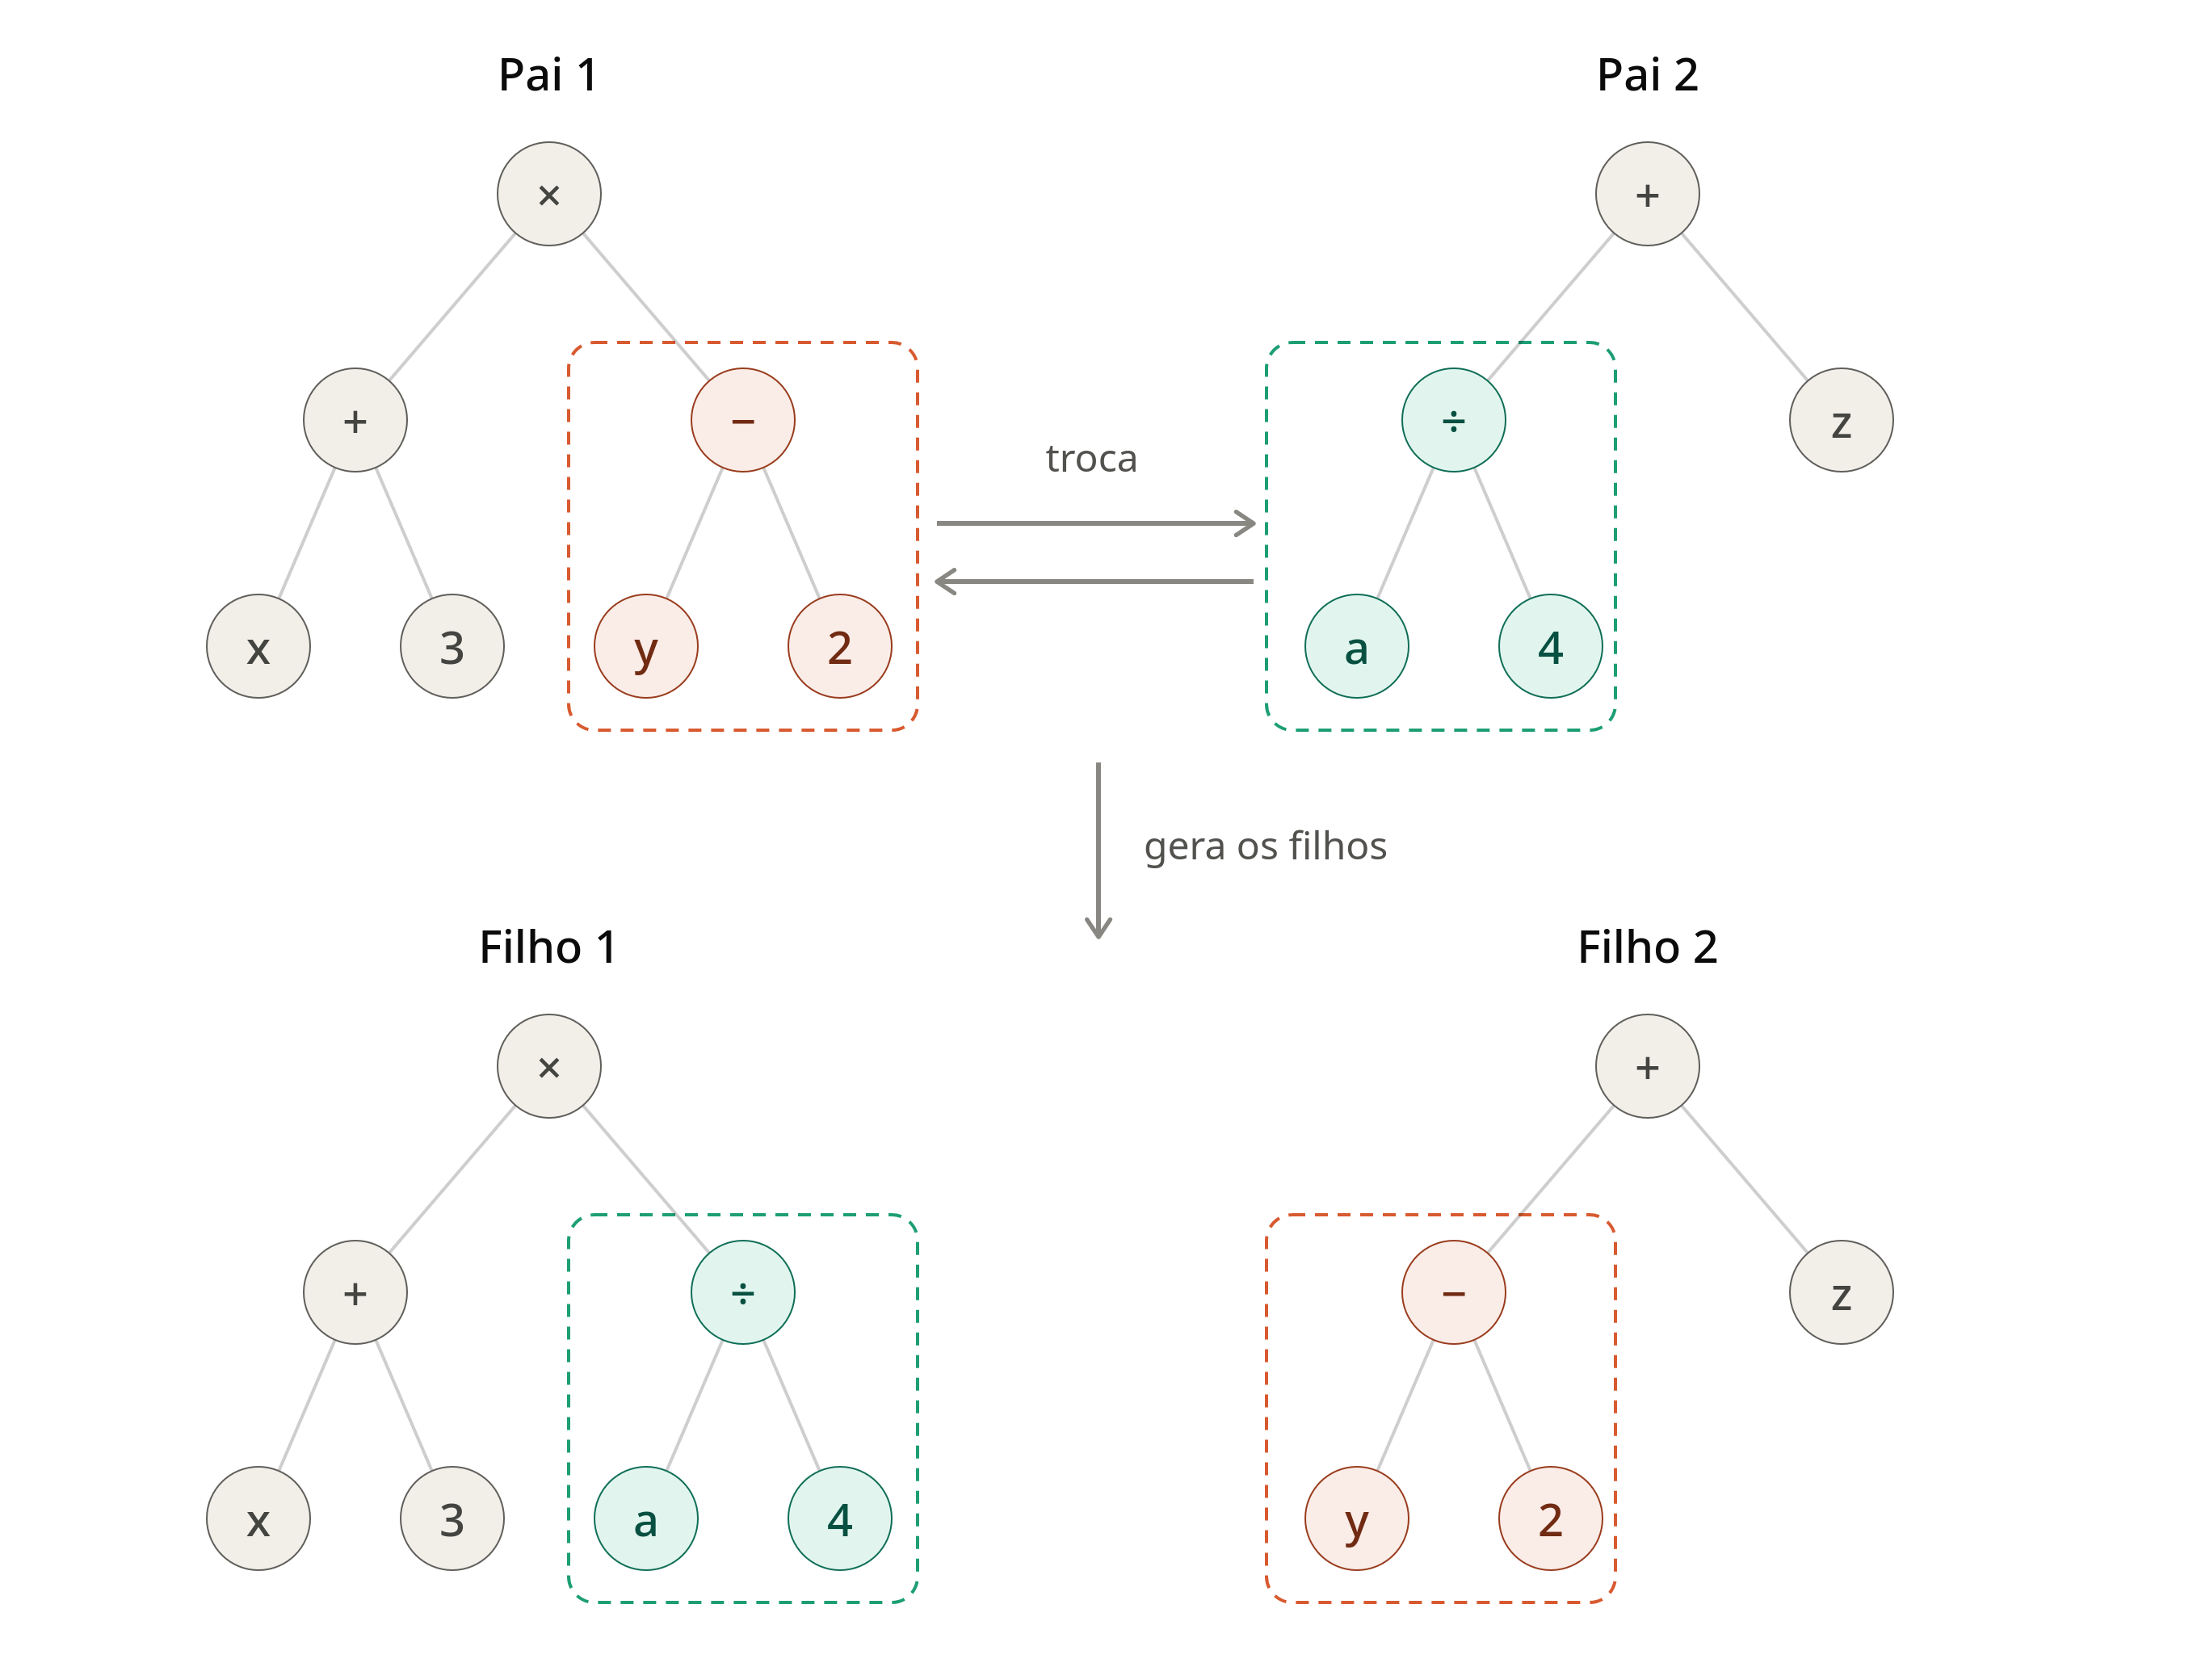
\includegraphics[width=\linewidth]{imgs/crossover.png}
          \caption{Operador de \textit{crossover}. Adaptado de \cite{koza1994}}
          \label{fig:cx}
      \end{figure}
    \end{column}

    \begin{column}{0.5\textwidth}
      \begin{figure}
          \centering
          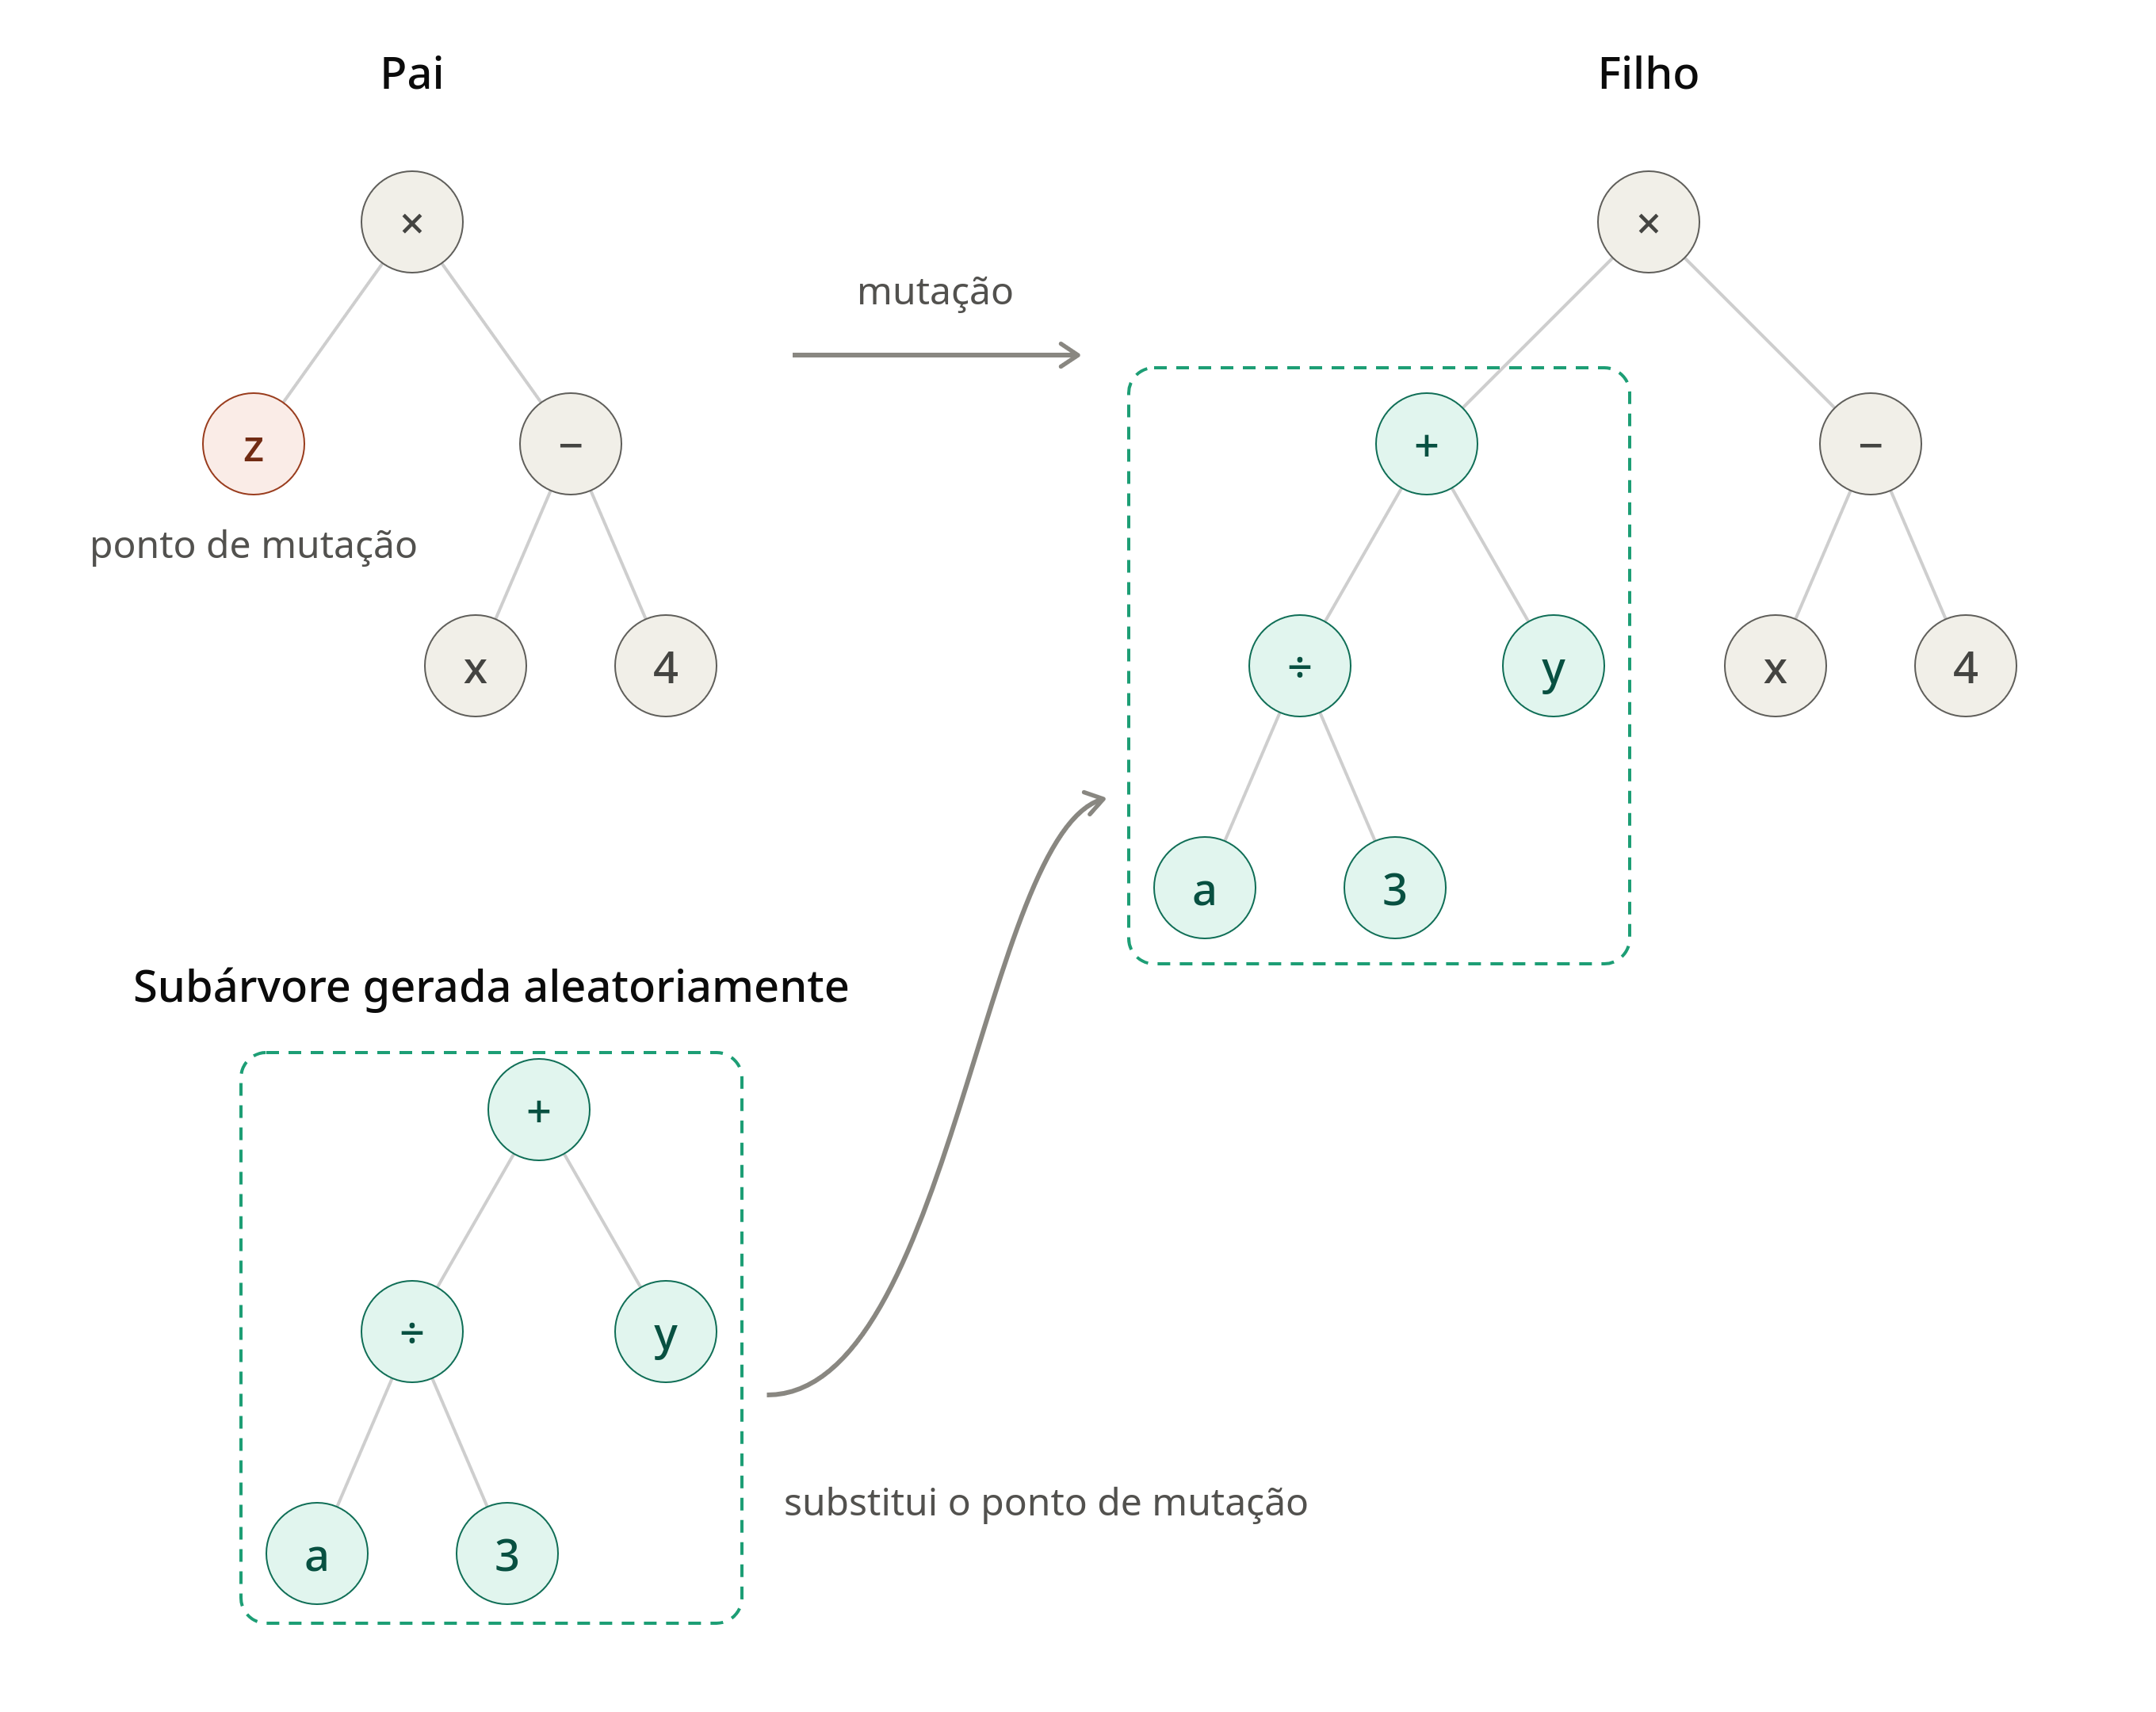
\includegraphics[width=\linewidth]{imgs/mutacao.png}
          \caption{Operador de mutação. Adaptado de \cite{fieldguide}}
          \label{fig:mut}
      \end{figure}
    \end{column}
  \end{columns}
\end{frame}

\subsection{\textit{General Program Synthesis Benchmark Suite}}
\begin{frame}{\textit{General Program Synthesis Benchmark Suite}}
  \begin{itemize}
    \item O \textit{General Program Synthesis Benchmark Suite}, ou PSB1,
      é um \textit{benchmark} que visa nivelar a avaliação de algoritmos de GP \cite{psb1}.
    \item Hoje muito usado na área \cite{psb2}.
    \item Problemas retirados de livros didáticos de introdução a computação.
    \item Especificação: exemplos.
  \end{itemize}
\end{frame}
\begin{frame}{\textit{General Program Synthesis Benchmark Suite}}
  \begin{examples}
    \textbf{Checksum:} dada uma string, converta cada caractere na string em
    seu valor ASCII inteiro, some-os, tome a soma módulo $64$,
    adicione o valor do inteiro correspondente ao caractere de espaço,
    e então converta esse inteiro de volta ao seu caractere correspondente
    (o caractere de \textit{checksum}).
    O programa deve imprimir \texttt{Check sum is X},
    onde $X$ é substituído pelo valor correto do caractere de \textit{checksum}.
  \end{examples}
\end{frame}
